\documentclass[16 pt]{amsart}
\usepackage{amscd,amsmath,amsthm,amssymb}
\usepackage{enumerate,varioref}
\usepackage{epsfig}
\usepackage{graphicx}
\usepackage{mathtools}
\usepackage{tikz}
\usetikzlibrary{graphs,arrows,topaths}
\newtheorem{thm}{Theorem}
\newtheorem{cor}[thm]{Corollary}
\newtheorem{lem}[thm]{Lemma}
\newtheorem{prop}[thm]{Proposition}
\theoremstyle{definition}
\newtheorem{defn}[thm]{Definition}
\theoremstyle{remark}
\newtheorem{ex}[thm]{Example}
\newtheorem{rem}[thm]{Remark}
\numberwithin{equation}{subsection}
\newcommand{\R}{\mathbb{R}}
\newcommand{\Z}{\mathbb{Z}}
\newcommand{\C}{\mathbb{C}}
\newcommand{\Q}{\mathbb{Q}}
\newcommand{\lh}{\lim_{h\rightarrow 0}}
\begin{document}

\title{Exam 2 Maths 140 Spring 2015 \\ DePaul University\\Dr. Alexander}
\maketitle
You have 90 minutes to complete this exam.  Calculators are allowed, but no other electronic devices are permitted.  Please write all your answers in complete, legible sentences, and show all your work to receive full credit.  There are seven (7) problems here.  You may choose to do any 6 of them.  
\vspace{1in}


%table
\begin{center}
  \begin{tabular}{ c | c }
    Problem & Score\\
    \hline
    &\\
    1&\\
    &\\
    2&\\
    &\\
    3&\\
    &\\
    4&\\
    &\\
    5&\\
    &\\
    6&\\
    &\\
    7&\\
    &\\
    Bonus&\\
    &\\
    \hline 
    &\\    
    Total& 
 \end{tabular}
\end{center}

\newpage 
Problem 1. Prove the following statement or give a counterexample:

Given any integer $n$, its square $n^2$ can be written in the form $4k$ or $4k+1$ for some integer $k$.





\newpage
Problem 2. Prove or disprove the following statements:

(a) Given two rational numbers $r_1$ and $r_2$ the power $r_1^{r_2}$ is also rational.\\

(b) Given two irrational numbers $s_1$ and $s_2$ their sum is irrational.


\newpage

Problem 3. Consider the following graph:

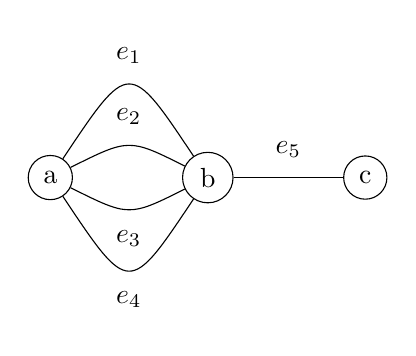
\begin{tikzpicture}
[scale=2,auto=left,every node/.style={circle}]
\node[circle,draw] (a) at (0,0){a};
\node[circle,draw] (b) at (1,0){b};
\node[circle,draw] (c) at (2,0){c};
\draw (a)..controls(.5,.25).. (b)node[midway,above]{$e_2$};
\draw (a)..controls(.5,-.25)..(b)node[midway,below]{$e_3$};
\draw (a)..controls(.5,.75)..(b)node[midway,above]{$e_1$};
\draw (a)..controls(.5,-.75)..(b)node[midway,below]{$e_4$};
\draw (b) -- (c) node[midway, above] {$e_5$};;
\end{tikzpicture}


(a) How many paths from a to c?\\

(b) b. How many trails from a to c?\\

Hint: Paths may not repeat vertices, trails may not repeat edges. 

\newpage

Problem 4.  Let $ A= \begin{bmatrix}
1 & 1 & 2 \\ 1 & 0 & 1 \\ 2 & 1 & 0
\end{bmatrix}$ 
(a) Find $A^2$, $A^3$.\\

(b) Let $G$ be a graph with three vertices and adjacency matrix $A$.  Draw $G$.\\

(c) Find $(A^2)_{1,3}$ Label the walks on your graph which match this.


\newpage

Problem 5. Does this graph have an Euler(ian) circuit, or a Hamilton(ian) circuit? If so give an example.  If not, explain why not.

\vspace{.25in}
\begin{center}


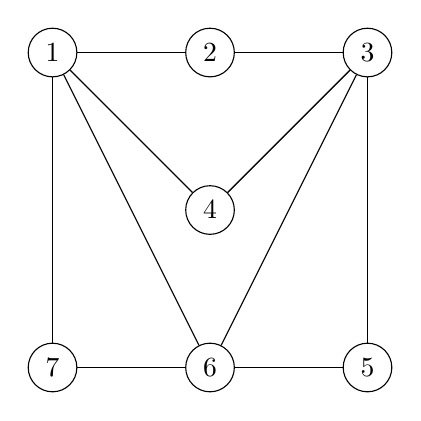
\begin{tikzpicture}
\node[circle,draw] (1) at (0,4){1};
\node[circle,draw] (2) at (2,4){2};
\node[circle,draw] (3) at (4,4){3};
\node[circle,draw] (4) at (2,2){4};
\node[circle,draw] (5) at (4,0){5};
\node[circle,draw] (6) at (2,0){6};
\node[circle,draw] (7) at (0,0){7};
\foreach \from/\to in {1/2,2/3,3/4,3/5,3/4,5/6,1/4,1/6,1/7,3/6,6/7}
  \draw (\from) -- (\to);
\end{tikzpicture}

\end{center}

\newpage

Problem 6. Does this graph have an Euler(ian) circuit, or a Hamilton(ian) circuit? If so give an example.  If not, explain why not.

\vspace{.25in}
\begin{center}
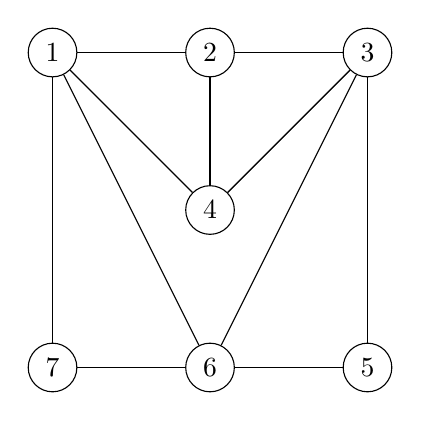
\begin{tikzpicture}
\node[circle,draw] (1) at (0,4){1};
\node[circle,draw] (2) at (2,4){2};
\node[circle,draw] (3) at (4,4){3};
\node[circle,draw] (4) at (2,2){4};
\node[circle,draw] (5) at (4,0){5};
\node[circle,draw] (6) at (2,0){6};
\node[circle,draw] (7) at (0,0){7};
\foreach \from/\to in {1/2,2/3,3/4,3/5,3/4,5/6,1/4,1/6,1/7,3/6,6/7,2/4}
  \draw (\from) -- (\to);
\end{tikzpicture}

\end{center}

\newpage

Problem 7. Draw the two graphs: $K_6$ and $K_{4,3}$.  What is the total degree of each?

\newpage

Bonus: Since a matrix is in some (reasonable) sense a two-dimensional analog of a number we can perform most of the operations on matrices in partly the same way as we can with numbers.  Of course, the matrices must be square, but there are even ways to get around this.  However, with more dimensions comes more solutions.  For example:
\[
\begin{bmatrix}
0&1\\1&0
\end{bmatrix}^2 = \begin{bmatrix}
1 & 0\\ 0 & 1
\end{bmatrix}
\]

So it could be reasonably said that this is a square root of the identity.  Since the matrix on the right functions in almost every way like th two-dimensional analog to the number one, we call it the identity.  How many ``square roots" are there to the $2\times 2$ identity matrix?

\end{document}